%\usepackage{biblatex}

\begin{document}

	
	
\title{ELEN2004/ELEN2020 Software Development I -- Report \\ Snakes And Ladders}

\author{Madiga Sehlapelo , 2321753}
\maketitle 
%\thispagestyle{empty}
\pagestyle{fancy}
\fancyhf{}

\fancyhead[R]{\thepage}
\fancyhead[L]{ELEN2004/ELEN2020 Software Development I Assignment}
%\vskip 3mm 
\pagenumbering{roman}

\newpage

\vspace*{\fill}
\begin{center}
	\begin{minipage}{.8\textwidth}
		\section*{Abstract}
		\addcontentsline{toc}{section}{Abstract}
		In this report I will discuss the design of a board game, snake and ladders. Snakes and Ladders is a very old board game invented in the 13th Century AD  by Saint Gyandev or so is believed by some historians. The purpose of this report is to illustrate one of many ways in which one can design the game's board. In the report I will go in depth in explaining how the game is played, what are the rules for winning and what are the rules for the game ending if there isn't a winner.
	\end{minipage}
\end{center}
\vfill % equivalent to \vspace{\fill}


\newpage
\tableofcontents
\newpage
 
\begin{center}
	\textit{This page is intentionally left blank}
\end{center}


\pagenumbering{arabic}
\newpage
\section*{Introduction}
\addcontentsline{toc}{section}{Introduction}
\subsection*{Snakes And Ladders}
\addcontentsline{toc}{subsection}{Snakes And Ladders}
Snakes and ladders is a multiplayer board game on a grid with dimensions ($n$,$n$). It is played using a 6 sided die, the rolled number on the die determines the number of moves one can should take. The goal is to reach get to the last block of the board. To continue with the explanation of the game, I will use an example. \\ \\
Take for example a $10\ by\ 10$ grid numbered from $1$ to $100$ in order. To make things a little bit more interesting, let us look at the game as a stage of life where one is working towards attaining financial success or any other type of success for that matter. One will need to roll a die to move, the rolling of the die represents chance that one gets and is independent of work put in. The board consist of snakes and ladders at certain blocks of the grid. When one lends on the base of the ladder, one moves up to the top of the ladder, and when one lend on the head of the snake, one moves to the tail of the snake. The snake can signify all the things that can take you back in terms of not attaining the success you want,god forbid, like losing a family member and the ladder on the other hand can signify entities that help you escalate quicker than luck can, things like me getting good grades for this assignment and increasing my chances of passing the course. No player can go down a ladder if the land at the top of the ladder. Each player plays in rounds, a round for a player will only change given that it is another players turn. This means that rolling again before another player plays or going up the ladder or being eaten by a snake doesn't increase nor decrease the rounds you've played. Each player can only roll again within the same round provided that the previous roll landed on a 6. In the context of the problem we are trying to solve, each player can only have a number of rounds equal to the number of blocks in the grid, in the case of our example, each player can only have a 100 rounds to play. If every player in the game has played all their 100 rounds and non has reached the end, if the is one leading player, he is considered the winner otherwise the game is terminated with a draw.\\
That is how the game works in a nutshell.

\section*{Board and Game Design}
\addcontentsline{toc}{section}{Board and Game Design}
The number of snakes and ladders are dependent on the binary encoding of my student number with the least significant digit on the right. The number of \textbf{0}'s represent the number of snakes and the number of \textbf{1}'s represent the number of ladders. \textbf{1000110110110101011001000} is the encoding of my student number, I added 3 extra \textbf{0}'s at the end for reasons specified in the \textit{Considerations of design} subsection.

\subsection*{Possible game termination outcomes}
\addcontentsline{toc}{subsection}{Termination outcomes}
The game has one of three outcomes, either it is terminated by a single player reaching the last block on the grid and therefore winning the game, or the game is terminated by a player winning due to being on the leading position when each and every player's round reaches max, or the game terminates as a draw when more than one player are on the leading position. Testing for the final case is difficult as this depends purely on luck.

\subsection*{Considerations of design}
\addcontentsline{toc}{subsection}{Considerations of design}
Ideally we want the game to go as long as possible to afford us the chance of getting each of the outcomes above on different trials in the testing phase. As mentioned in the specifications, we wish to have more snakes than ladders, I therefore added 3 extra \textbf{0}'s in the encoding of my student number to achieve this. In addition to the number of snakes and ladders, I believe it is ideal to have most snakes be long while most ladders are short. One other non-trivial consideration is where should the snakes and ladders be placed on the board. We do not want to have most a lot of snake heads in one area which might make it impossible to move past that point, neither do we want to have to snake heads or two ladder bases on one block for obvious reasons.  

\subsection*{The Solution}
\addcontentsline{toc}{subsection}{The Solution}
The idea here is to use the object oriented design paradigm. In this paradigm, entities that are interacting are just objects.Each object has it's own attributes and functions. In this game we will have the following objects:
\addcontentsline{toc}{subsubsection}{Object Oriented Design}
\begin{itemize}
	\item \textbf{Player:} A player who's attributes might include but not limited to the player's position, player's recent/current round and whether they moved by snake, ladder or die roll. It's functions might be to roll or dice, to set the current state of the player etc. Each player will have their own die to roll, the idea is that each player should have a different seed to the random number generator. 
	\item \textbf{Snake and Ladder Objects:} I put this in the same bullet point as they serve the same purpose just in opposite directions. Like all other objects, these will have their own  attributes and functions as well. These will have the start positions and lengths as attributes and it's functions will be nothing but getters and setters.
	\item \textbf{Tile:} The tile object is probably my favorite designed object, a tile represents each block on the grid or board. The interesting part of the tile object is that each and every tile on the board will have a head of a snake as well as a base of a ladder. But recall that a snake or a ladder are just objects. the snakes and ladders will have a \textit{status} attribute, which just says whether that snake or ladder is active or not. An inactive snake or ladder will not affect any player and has length zero.
	\item \textbf{Board:} This is the biggest piece of the puzzle. The reason the board is an object of its own is because we can read in multiple boards from one file. Each board instance can be looked as the whole game. Each board will have a configuration of snakes and ladders on the board. As attributes, the board will have a list of players, a list of tiles ordered from to the size of the board, since the number of players and tiles is unknown before hand, a vector is the storage mechanism we are going to use to represent our list. number of players, number of snakes, number of ladders and size will also be attributes of the board object. The functionality of this object will include but not limited to, adding a snake and ladder of to the board, checking the current board status after every move to look for a winner and setting the winner of the game played on the current board object.
\end{itemize}

Each board can be seen as a game it self. The main section in the implementation will consist of three parts only and they will be as follow:


\begin{itemize}
	
	\item \textbf{Reading input:} I imagine it might be difficult to in interact directly with the input file. In this section, I will read in the file and store its contents into a list, where the list is a vector since we do not know how many lines are on the page. Each line will be an entry into the list. An blank line will not be read in to our list, therefore our detection mechanism for another board will be to detect if the next line is a starts with a number or not.
	\item \textbf{Boards initialization:} This is the next middle piece of the whole puzzle and very crucial, no mistakes can be afforded here. The idea here is that all boards that appear in the input file should be initialized way before the first game on the first board begins. Since every board is equivalent to a game as mentioned before, every board is stored into another list of boards or games and yes, a vector will be used as the storage mechanism or list. Every board will have its set amount of players and board configuration at the end of this stage. All that's left is for the games to begin.
	\item \textbf{Playing the game}: This is adding meat to the bones. At this point we've read in the data and initialized all the boards. The game will probably be run in a for loop for each board. We do do not know how many rounds will be played for each player or whether or not there will be a player. The idea then is to run the game as long as there is no winner or there's no draw, this functionality will be checked by the board object. Upon every single move a player makes, the move will be recorded in the output file as well as the relevant information about the current move made. Upon every move except being bitten by a snake, we should check the board or the game for a win so that we terminate as soon as a player wins the game. 
\end{itemize}
Upon playing the game, we proceed to the very next board if any exists, otherwise we terminate.
\addcontentsline{toc}{subsubsection}{The Three Phases}

\section*{Results}
\addcontentsline{toc}{section}{Results}
In this section I discuss the results that came from our codes in the form of tables. The results here are a result from boards that are designed by the student number as well as boards that are designed to check whether the code is able it give all possible outputs, namely, winning by finishing, winning by end of rounds and draw.

\subsection*{Results on boards designed from the student number}
\addcontentsline{toc}{subsection}{Student Number designed boards}
Below are tables for 3 separate trials. Here we expected a winner by finishing as there is a greater chance of that happening given any board. At first there are only 3 players to test if the code can handle multiple players. and the results are self-explanatory.\\ \\
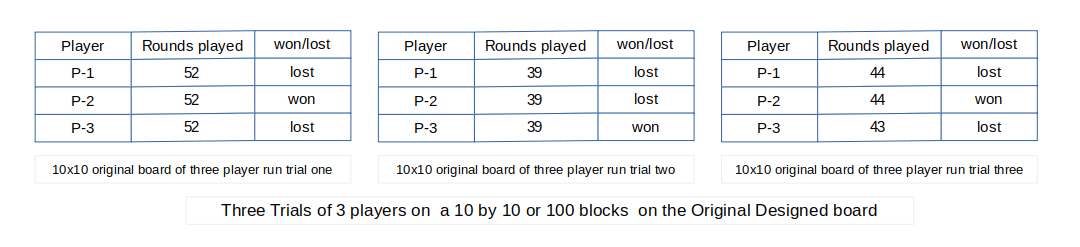
\includegraphics[scale=0.5]{threeOrig.png}\\\\
If you look at the input file, I have designed 2 boards of different sizes and different number of players. This is approximately double the size and double the amount of snakes and ladders but different lengths of course. In every trial we get different results which shows that the code to produce results purely based on luck or chance.\\
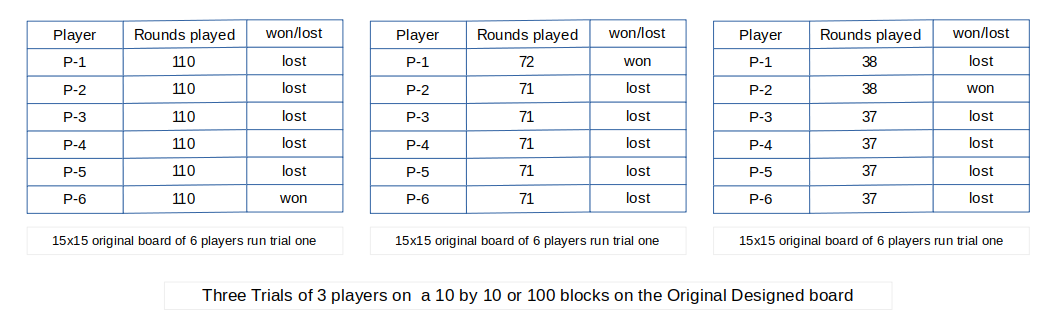
\includegraphics[scale=0.5]{sixOrig.png}\\

\subsection*{Results on boards designed to test conditions of winning}
\addcontentsline{toc}{subsection}{Testing purpose designed boards}
In this section we doctored the design of the boards and the snakes were not purely random. there are two tables as well like we had in the above subsection. The aim was to show find out whether we can achieve a draw. The game board therefore reaches a point where there are 6 consecutive snakes that have the same tail point. This then means at some point all players in the game will get stuck at a single point until they run out of rounds. As a result, both the left most tables have draws. In the middle and right most table, we made it impossible pass a certain point and by adding 6 consecutive snakes but different tail points. That way all players get stuck in the game and the winner is decided by having lead in the game.\\
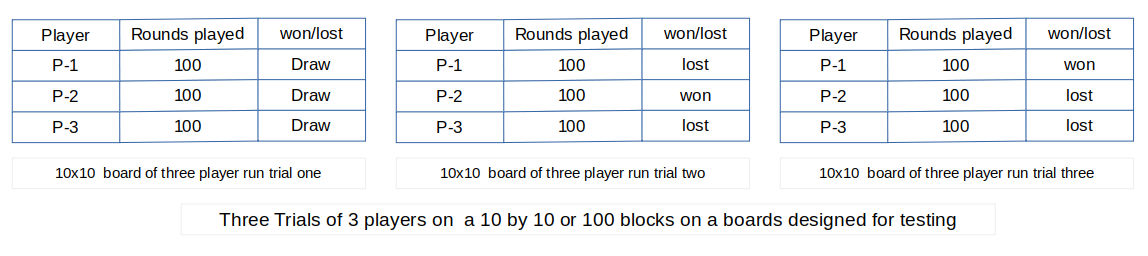
\includegraphics[scale=0.45]{three.png}\\
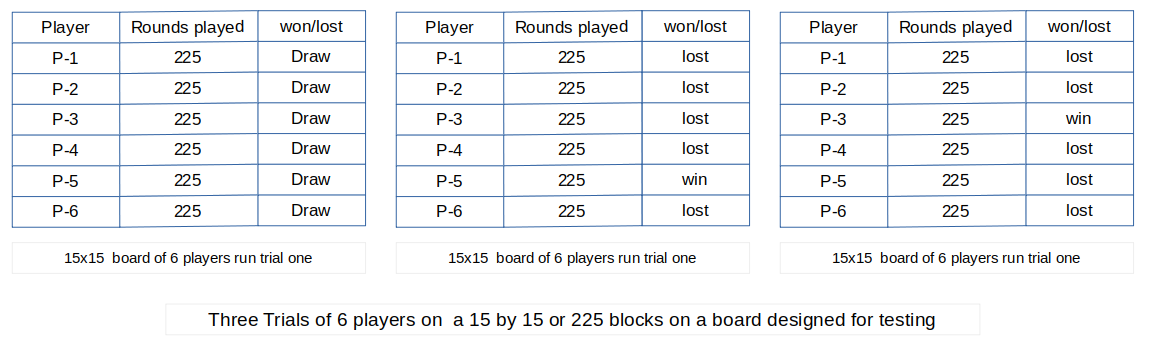
\includegraphics[scale=0.45]{six.png}\\ 
Here we can then deduce that upon many trials and most of which are not included in the report, we can confidently say that our implementation and design is a perfect solution in terms of functionality. In terms of performance and maintainability, this could be arguable but I am quite confident that this could be way far from the worst solution to the problem.

\section*{Discussion}
\addcontentsline{toc}{section}{Discussion}
\subsection*{The Approach}
\addcontentsline{toc}{subsection}{The Approach}
The aim is to complete a given task by minimizing the amount of code one will write. Having this in mind and upon reading the requirements/specifications document, the objected oriented approach made the most sense to achieve the goal. This reason I went with this approach was to ensure consistency within similar entities of the i.e. I do don't have to worry about changing players characteristics individually. This approach also saves us a huge amount of redundant code.
\subsection*{The Solution}
\addcontentsline{toc}{subsection}{The Solution}
Like every game, the aim is to have while playing it, but there's is no fun in a game which is easy or very difficult to win. The element of chance makes it unpredictable to an extent, but the lengths of the snakes and ladders are what we can control to measure the fun players can have. The length of snakes was informed the idea that sometimes when life knocks you, it knocks you so hard that it takes you back to where you started from. The ladders on the other hand, their lengths depict how slow one moves to attain the success they need. The whole idea however is that psychologically, people tend to be interested in things they relate to. Therefore, making our solution depict the real world made sense even though the players is just a processors adding 1's and 0's in the background playing against itself.
\subsection*{Improvements and Validations}
\addcontentsline{toc}{subsection}{Improvements and Validations}
I can not think of any improvements I would have made in terms of the overall performance of the implemented solution. One improvement I could have made is in terms of reducing the amount of code I wrote by making the snake and ladder object as one object. This makes it easy to keep the code maintained. The reason why this improvement could have been made is because of the fact that the snake and the ladder does the exact same job just in opposite direction. The problem with the current implementation is that if I add a function to the snake class, I need to add the exact same function to the ladder class.\\
One more improvement I could have added is dynamically creating the input of snakes and ladders and the writing it to a file. This would cut off the dependency on input file which I believe could be outside the scope of this assignment, or maybe not. \\ \\
This assignment wasn't at all easy, the only assumptions that were made were ones in relation to the time taken to complete the project. Having played the game before many times and understanding how it works, I assumed I would have completed it sooner that I did but I didn't, and that's okay because life is like rolling a 1 and landing on the head of snake and not get what you want sometimes. 

\section*{Conclusion}
\addcontentsline{toc}{section}{Conclusion}
All boxes have been checked, code works exactly as intended, or so I believe. There are many design patterns one could have employed, the object oriented design made it significantly easier to implement the solution than just sequentially writing code that is prone to having intractable bugs. Relating life events to the game of snake and ladders also helped in keeping me motivated to get to the finish line.

\newpage
\section*{References}
\addcontentsline{toc}{section}{References}
\bibliography{ref}
[1] \ \ \ \ \ \ \ \ \ \ \   \href{http://www.cplusplus.com/reference/}{C++ Reference }

[2] \ \ \ \ \ \ \ \ \ \ \   \href{geeksforgeeks.org}{Geeks For Geeks, Programming with C++}

[3] \ \ \ \ \ \ \ \ \ \ \   \href{https://www.overleaf.com/learn/latex/Bibliography_management_in_LaTeX#Further_reading}{Stack Overflow Error finding and debugging}

[4] \ \ \ \ \ \ \ \ \ \ \   \href{https://www.programiz.com/cpp-programming}{Programming with C++ site:Programiz}

\newpage
\section*{Appendix}
\addcontentsline{toc}{section}{Appendix}

\subsection*{A: Project Time Management}
\addcontentsline{toc}{subsection}{A: Project Time Management}

\newpage
\subsubsection*{B: Flow Chart}
\addcontentsline{toc}{subsection}{B: Flow Chart}
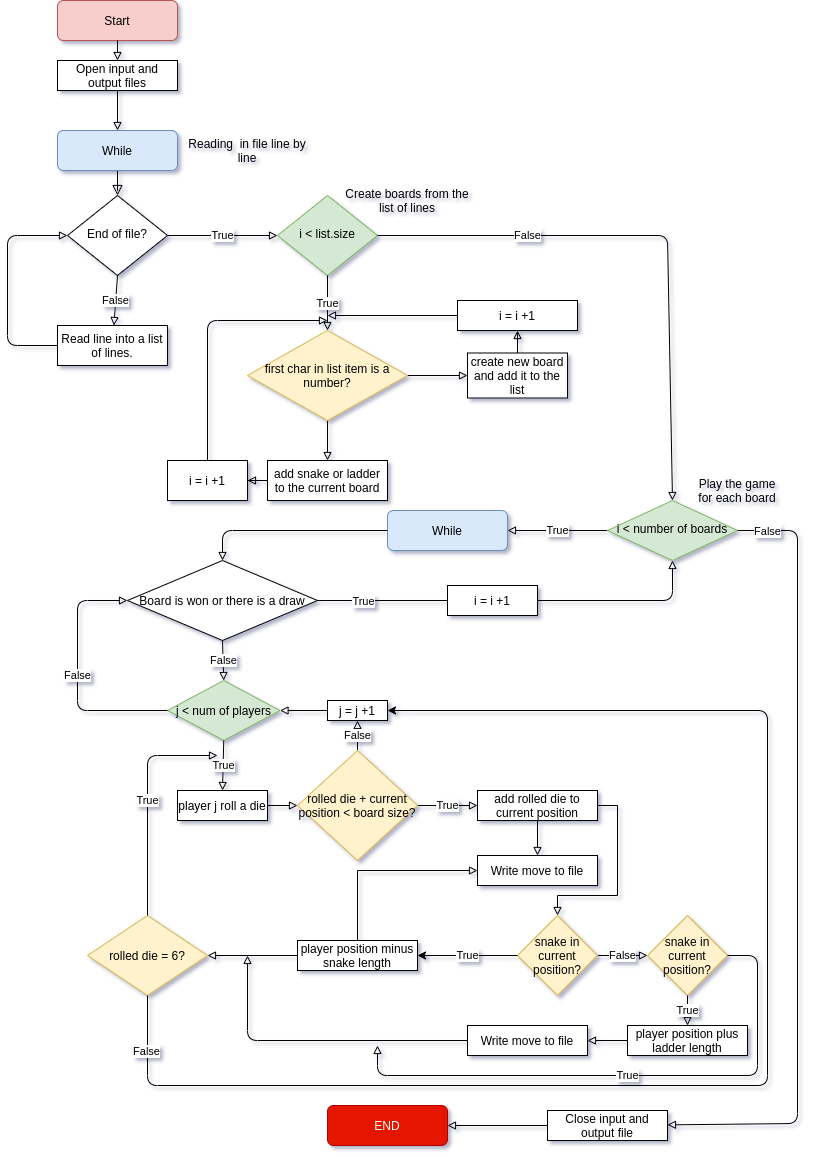
\includegraphics[scale=0.5]{SnL.png}



\end{document} 

